\chapter{Elaboration of the realization of the approaches}

This section discusses the optimization of the two service scans from the previous section, each using a different approach. In addition, the third approach discussed is to avoid scanning unsupported services.

\section{Reuse information within same service}

This approach aims to reuse information from one part of a service for another part of this service. First, it must be checked to which service this approach should be applied to.

\subsection{Choosing the RC service to apply the approach to}

This approach is applicable to scans of services with multiple parameters, as it is the case for the Routine Control (RC) service. It has two parameters, the routine type and the routine identifier (more in \autoref{subsubsec:uds-services}). The distribution of the identifiers is visualized grouped by the type as a histogram in \autoref{fig:rc-distribution}.

\begin{figure}[htb]
    \centering
    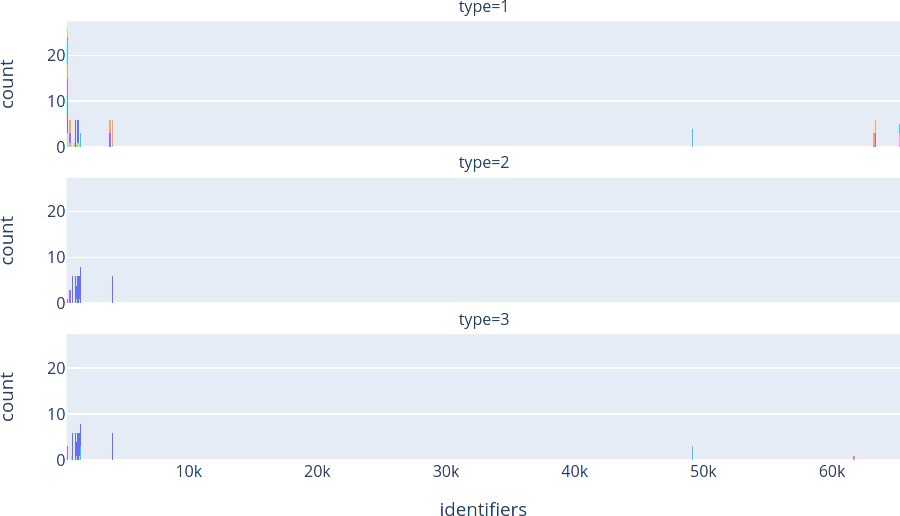
\includegraphics[width=0.8\textwidth]{rc-distribution}
    \caption{Distribution of the RC identifiers. Each color is one ECU.}
    \label{fig:rc-distribution}
\end{figure}

It can be seen that if an identifier is available in type1, it is likely that this identifier also occurs in type2 or type3. Consequently, if an identifier does not respond positively in type1, it is unlikely that it will respond in type2 or type3.

Hence, the RC service is a great candidate for this approach.

\subsection{Current behavior}

There are three control types, and because the identifier field has a length of 16-bits, there are 2\textsuperscript{16} identifiers. This leads to the following formula, showing how many requests are generated for a UDS scan:
\[f(n)=3 \cdot 2^{16} \cdot n\]
wherein $n$ stands for the number of detected states.

The current RC scan does exactly this, it generates the full range for each state. Its current behavior is illustrated in \autoref{fig:rc-behavior-current}. The green areas symbolize the scanned ranges.

\begin{figure}[htb]
    \centering
    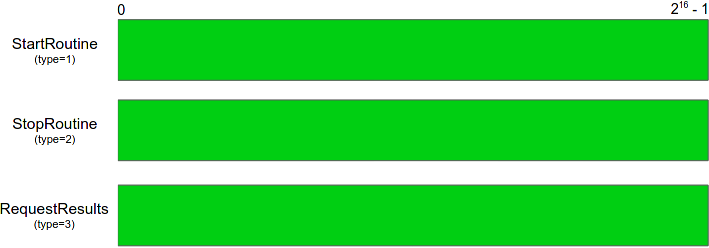
\includegraphics[width=0.8\textwidth]{rc-behavior-current}
    \caption{Current behavior of the RC service scan.}
    \label{fig:rc-behavior-current}
\end{figure}

\subsection{Elaborating the new behavior}
\label{subsubsec:rc-elaborating}

The new behavior starts with scanning all 2\textsuperscript{16} identifiers with type1. Only the identifiers, which led to a positive response, are scanned with type2 and type3 as well. So, 2\textsuperscript{16} is the new minimum number of requests for each state for this service, resulting in an upper limit of request savings of 66.7 \%.

It was observed that there seems to be a locality effect for the identifiers. Thus, if an identifier with type1 is answered positively, scanning also nearby identifiers for type2 and type3 results in higher coverage. To exploit this, an expansion width is introduced. This width specifies how a single value is expanded to a range in both directions. For example, with an expansion width of 100, the value 1500 would be expanded to the range 1400 – 1600.

\autoref{fig:rc-behavior-new} illustrates the new behavior. The green areas again show the scanned ranges. In addition, the red areas are the found identifiers in type1 and their resulting scans for type2 and type3. The gray areas show the routine identifiers not requested with this new behavior.

\begin{figure}[htb]
    \centering
    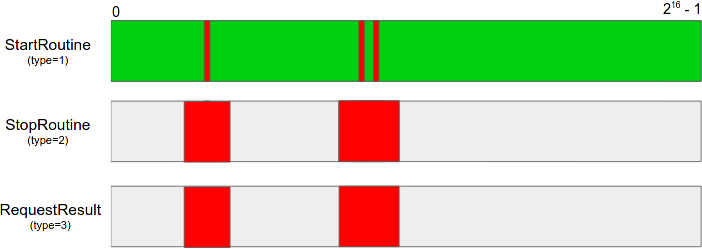
\includegraphics[width=0.8\textwidth]{rc-behavior-new}
    \caption{New procedure for scanning the RC service.}
    \label{fig:rc-behavior-new}
\end{figure}

What needs to be found out is the expansion width which leads to the best coverage, while maintaining an appropriate request saving. For this, scans with different expansion widths were simulated. These simulations work based on the information gathered from the real ECUs as described in \autoref{sec:data-gathering}. For a quick simulation another observation is used. If an identifier is available in a state, it is likely to be available in the other states too. Thus, the states are ignored in the simulation, which improves the performance by a multiple, while it is still close to the real ECUs. The required information, which identifiers are supported by an ECU for which type, is extracted from the generic.log files.

As described, the simulation starts with getting all identifiers which have been positively answered by the currently simulated ECU. Subsequently, these identifiers are expanded to both sites from 0 to 1000. Overlapping ranges are resolved to a continuous space. The sizes of the resulting ranges lead to the theoretically generated requests which can be calculated to the coverage and request saving. These values of all ECUs are averaged to the final result.
 
The pseudocode of \autoref{lst:rc-sim} shows the procedure more clearly.

\begin{listing}[H]
\begin{minted}
[frame=single,
framerule=0pt,
framesep=2mm,
baselinestretch=1.2,
bgcolor=VeryLightGray,
fontsize=\footnotesize,
linenos]
{python}
coverages = []
request_savings = []
for expansion_width in range(1001):
    coverages_width = []
    request_savings_width = []
    for ecu in ecus:
        ids_type1 = get_type1_ids(ecu)
        to_scan = ids_to_block(ids_type1, expansion_width)
        count_requests = len(to_scan)
        coverages_width.append(get_coverage(ecu, to_scan))
        request_savings_width.append(get_saving(count_requests))
    coverages[expansion_width] = avg(coverages_ecus)
    request_savings[expansion_width] = avg(request_saving)
\end{minted}
\caption{Simulation procedure for finding the best expansion width.}
\label{lst:rc-sim}
\end{listing}

The result of this simulation is plotted in \autoref{fig:rc-simulation-result}. The request saving is almost linear to the expansion width. That makes sense, because the larger the expansions are, the more requests are generated. The expansion width of zero represents the results without using the locality effect.

\begin{figure}[htb]
    \centering
    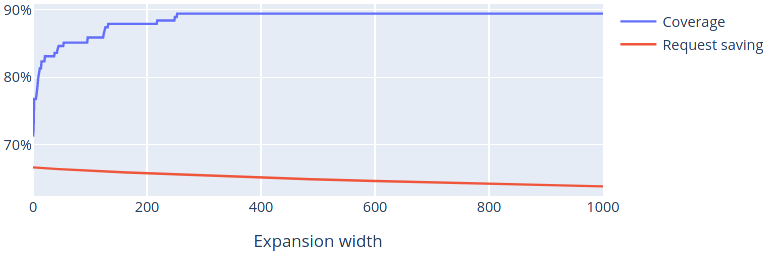
\includegraphics[width=0.8\textwidth]{rc-simulation-result}
    \caption{Result of the RC scan simulation to find the best expansion width.}
    \label{fig:rc-simulation-result}
\end{figure}

Since the request saving decreases only slowly, the highest coverage was chosen, which starts with the expansion width \textbf{253}. Hence, this value is the chosen and implemented one.

The simulations were also run with expanding identifiers in one direction only, which yielded very similar results. Thus, it was left in both directions.


\section{Use probabilities of positive answers block based}

Most services are simpler and only have one parameter. So, reusing information within the same service is not practical. This approach tackles these kinds of services. The new idea is to scan the blocks more heavily where positive behavior is more likely than others and vice versa.

\subsection{Choosing the RDBI service to apply the approach to}

The Read Data By Identifier (RDBI) service has only one parameter, the identifier of the requested data.

The distribution of positively answered identifiers over all ECUs is visualized in a histogram to check if there is potential. The result can be seen in \autoref{fig:rdbi-distribution}.

\begin{figure}[htb]
    \centering
    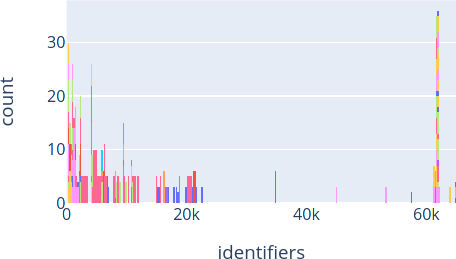
\includegraphics[width=0.7\textwidth]{rdbi-distribution}
    \caption{Distribution of the RDBI identifiers. Each color is one ECU.}
    \label{fig:rdbi-distribution}
\end{figure}

It is clearly visible that there are some areas where not a single identifier was answered positively, and some areas that are particularly covered, such as the beginning and the end. This behavior of the RDBI will be exploited in the remainder of this section.

\subsection{Current behavior}

As for the RC service, the identifier field has a length of 16-bits. Hence, there are 2\textsuperscript{16} possible identifiers.
The current RDBI scan is simple. It generates 2\textsuperscript{16} requests counting up from 0 to 65,535 as the identifier. This leads to the following formula, showing how many requests are generated for a UDS scan:
\[f(n)=2^{16} \cdot n\]
wherein $n$ stands for the number of detected states. 

\subsection{Elaborating the new behavior}
\label{subsubsec:rdbi-behavior}

To reduce this range, first the 2\textsuperscript{16} area is divided into blocks. For each block a specific number of requests is generated. If any of these requests is answered positively, the whole block is scanned.  An example is illustrated in \autoref{fig:rdbi-behavior-new}.

\begin{figure}[htb]
    \centering
    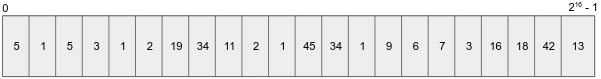
\includegraphics[width=0.7\textwidth]{rdbi-behavior-new}
    \caption{New procedure for scanning the RDBI service.}
    \label{fig:rdbi-behavior-new}
\end{figure}

The first point to answer is how the number of requests is calculated for each block. It is based on the probability of positive identifiers of this block. This probability is gathered from merging all positively answered identifiers of all ECUs and then for each block calculating $\frac{occurences}{block\_size}$. The number $r$ of requests for a block is calculated with
\[r(i, s)=\max(p(i, s) \cdot s, 1)\]
wherein $p$ stands for the probability function, $i$ for the index of the requested block and $s$ for the block size. For each block should be generated at least one request. The requested identifiers within a block are generated randomly.

The second question is which block size leads to the best results. This is again answered by a simulation. As potential block sizes $2^2, 2^3, ..., 2^{15}, 2^{16}$ were chosen because they are divisors for 2\textsuperscript{16}. The resulting coverages and request savings are then calculated for each ECU specifically and averaged to the final result. Same as for the RC service, the states are ignored in the simulation.

The approach has a feature which makes the simulation more complex than the former simulation. Since the blocks are first scanned randomly, the scan can lead to a great coverage, but also a low one, depending on the hit rate of the generated identifiers. To reduce this effect, the simulation is made 100 times, each time with newly created random identifiers. The 100 results are averaged to the coverage and request saving corrected from the random factor. This leads to a high processing time. To reduce the runtime, the execution was parallelized.

The pseudocode of \autoref{lst:rdbi-sim} shows the procedure more clearly.

\begin{listing}[H]
\begin{minted}
[frame=single,
framerule=0pt,
framesep=2mm,
baselinestretch=1.2,
bgcolor=VeryLightGray,
fontsize=\footnotesize,
linenos]
{python}
coverages = []
request_savings = []
for exponent in range(2, 17):
    block_size = 2 ** exponent
    probabilities = get_probabilities(ecus, block_size)
    coverages_block = []
    request_savings_block = []
    for ecu in ecus:
        for i in range(100):
            req_random = random_samples(block_size, probabilities)
            positive_identifiers = ecu.get_positive_identifiers(req_random)
            req_block = to_blocks(positive_identifiers, block_size)
            positive_identifiers = ecu.get_positive_identifiers(req_block)
            count_reqs = len(samples) + len(req_list)
            coverages_block.append(get_coverage(ecu, positive_identifiers))
            request_savings_block.append(get_saving(count_reqs))
    request_savings[exponent] = avg(request_savings_block)
\end{minted}
\caption{Simulation procedure for finding the best block size.}
\label{lst:rdbi-sim}
\end{listing}

This simulation leads to \autoref{fig:rdbi-simulation-result}.

\begin{figure}[htb]
    \centering
    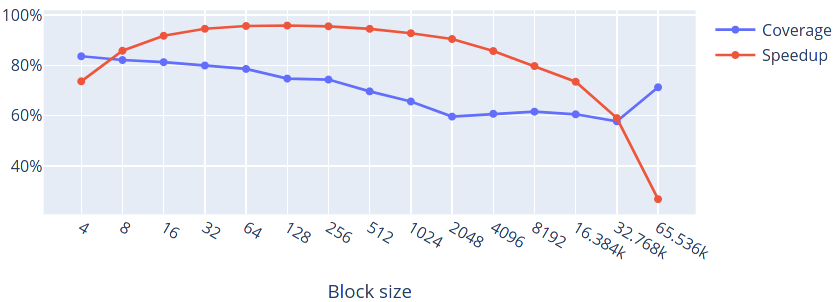
\includegraphics[width=0.8\textwidth]{rdbi-simulation-result}
    \caption{Simulation result for the RDBI service.}
    \label{fig:rdbi-simulation-result}
\end{figure}

The request saving is no longer linear; instead, it is highest for medium block sizes. From block sizes 64 to 128, the coverage decreases by 4\% while the request saving remains the same. Thus, it was decided for \textbf{64} as the block size leading to best results.


\section{Avoid the scan of unsupported services}
\label{subsec:unsupported-services-elaboration}

Each ECU usually supports only a subset of the services offered  by the UDS standard. This approach aims to avoid scanning them in order to save requests and therefore, time.

The first thing to understand is how to tell if a service is supported or not. The UDS standard defines the general server response behavior, shown in \autoref{fig:server-response-behaviour} with the important area highlighted.

\begin{figure}[htb]
    \centering
    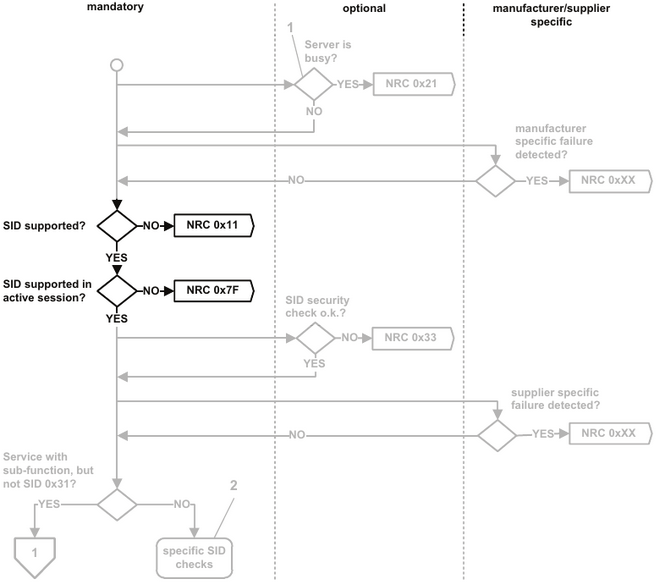
\includegraphics[width=0.8\textwidth]{server-response-behaviour}
    \caption{General server response behavior \cite{iso14229}. SID = service identifier.}
    \label{fig:server-response-behaviour}
\end{figure}

Each request is answered by a response, either positive or negative. A negative response contains a negative response code (NRC). \autoref{fig:server-response-behaviour} shows that the NRCs 0x11 and 0x7f are relevant for this approach. 0x11 indicates that the requested service is not supported at all. 0x7f is a lighter response code because it shows that the requested service is not supported in the current state of the ECU. Both response codes are sufficient to stop the current service scan with the current state and start with the next one. Although a 0x11 NRC is received, this service is still probed in other states. This is because with this behavior, in the worst case, one request is generated for this service per state, which in turn receives 0x11 NRC again and then stops the service scan. The number of states detected is usually one-digit, so the number of requests generated is negligible. But in the best case the vendor has implemented the NRC incorrectly and the service is available in a different state.
